% !TEX encoding = UTF-8 Unicode
% !TeX spellcheck = it
\documentclass[a4paper,8pt]{article}
\usepackage[italian]{babel}
\usepackage{graphicx}
\usepackage{blindtext}
\usepackage[T1]{fontenc}
\usepackage[utf8x]{inputenc}
\usepackage{multicol, caption}
\usepackage[none]{hyphenat}
\usepackage{hyperref}
\usepackage{xcolor}
\usepackage[margin={2.5cm,3cm}]{geometry}
\usepackage{titlesec}
\usepackage{amsmath}
\usepackage{tabularx} % for 'tabularx' environment
\graphicspath{ {images/} }
\newenvironment{Figure}
  {\par\medskip\noindent\minipage{\linewidth}}
  {\endminipage\par\medskip}

\newenvironment{Table}
   {\par\bigskip\noindent\minipage{\linewidth}\centering}
   {\endminipage\par\bigskip}

\setlength{\columnsep}{1cm}

\hypersetup{
	colorlinks=true,
	allcolors=[rgb]{0.376,0.49,0.54}
	%urlcolor=[rgb]{0,0,0}
}

\titleformat{\section}
{\normalfont\fontsize{11}{11}\bfseries}
{\thesection.}{1em}{}

\titleformat{\subsection}
{\normalfont\fontsize{9}{9}\bfseries}
{\thesubsection.}{1em}{}

\begin{document}
\title{Comparazione di classificatori in Credit Card Approval}
\author{Valerio Colitta, Daniele Cominu, Alessio Fiorenza}
\date{Aprile 2017}
\maketitle

%TODO: inserire un indice con i vari link alle section.%

\begin{multicols}{2}

\section{Descrizione preliminare}
Volendo approfondire i metodi e le tecniche di classificazione affrontate nel corso di Metodi Quantitativi per l'Informatica, abbiamo deciso di confrontarli risolvendo il problema presentato in \emph{Credit Approval Data Set} \cite{Dataset}; abbiamo deciso di utilizzare modelli di diverse complessità ed abbiamo osservato che data la conformazione dei dati e la loro dimensione ridotta, si ottengono risultati migliori con modelli meno complessi. 

\section{Il dataset}
Il dataset riguarda delle domande di approvazione di carte di credito, ed e' composto da 690 campioni, 37 dei quali con valori mancanti. Sono presenti in totale 15 feature, le quali si articolano in 6 continue e 9 categoriche. Tali dati sono poi classificati in due classi \{+, -\} che rappresentano rispettivamente l'approvazione o meno della carta di credito.
Il significato delle 15 feature non è noto per poter mantenere la confidenzialità dei dati.

\section{Manipolazione dei dati}
Come prima cosa sono stati eliminati manualmente dal dataset i 37 campioni di cui non erano stati specificate alcune feature, riducendo ulteriormente la dimensione del dataset a 653 campioni.\\
\subsection{One Hot Encoding}
Per superare l'eterogeneità nella tipologia delle feature, si è deciso di applicare la tecnica del \emph{One Hot Encoding} \cite{OneHotEncoding} per le feature categoriche; l'\emph{One Hot Encoding} è una tecnica utilizzata per trattare feature categoriche in problemi di classificazione e regressione, e consiste nel tradurre una feature categorica che può assumere \emph{n} valori distinti in un vettore di \emph{n} feature binarie; per ogni campione la feature i-esima del vettore calcolato assume il valore 1 se e solo se il campione assume il valore i-esimo per la feature considerata; le restanti \emph{n }- 1 sono dunque settate a 0 per tale campione.
Se si fosse utilizzata una feature a valori reali, in cui per ogni valore assunto dalla feature viene associato un numero reale, sarebbero state introdotte delle distanze diverse tra i valori assunti dalla feature; Ad esempio, considerando una feature categorica che descrive la specie di appartenenza, mappando i valori assunti a dei numeri incrementali, si può notare come si introduca una maggiore distanza tra i campioni (2, 7) rispetto ai campioni (4, 5).
\begin{Figure}
 \centering
 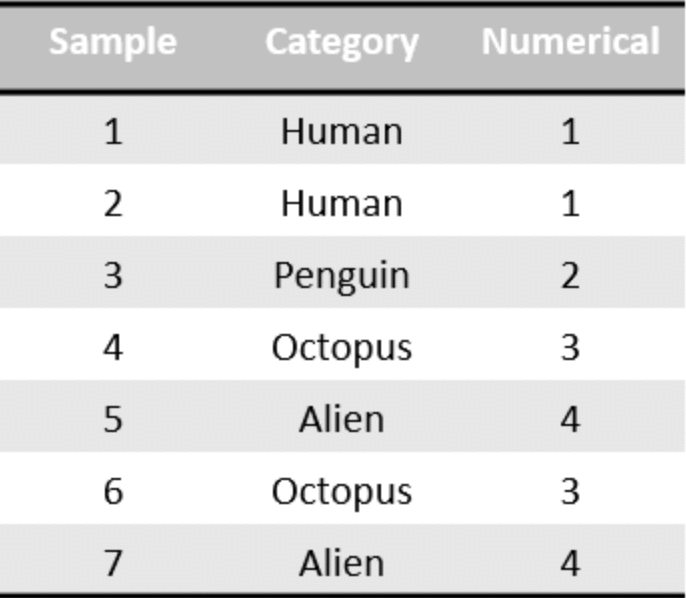
\includegraphics[width=\linewidth]{categbw}
 \captionof{figure}{mapping categorica -> reale}
\end{Figure}
Introducendo il one hot encoding si può notare come le distanze tra i campioni (2,7) e (4,5) siano le stesse\\
\begin{Figure}
 \centering
 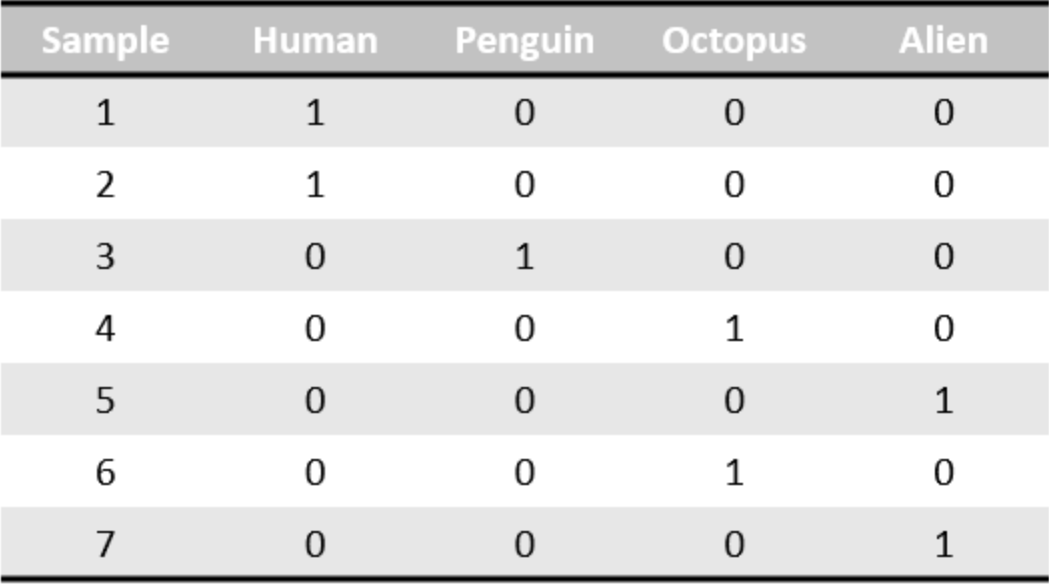
\includegraphics[width=\linewidth]{categvecbw}
 \captionof{figure}{one hot encoding}
\end{Figure}


\subsection{Standardizzazione}
Successivamente all'one hot encoding, è seguita la fase di standardizzazione delle variabili; per ogni feature sono stati calcolati la media campionaria $\mu$ e la deviazione standard campionaria $\sigma$, definite come: 
\begin{equation}
	\mu_{j} = \frac{1}{N}\sum_{i=1}^{N} x_{ij}
\end{equation}
 
\begin{equation}
	\sigma_{j} = \sqrt{\frac{1}{N-1}\sum_{i=1}^{N}(x_{ij} - \mu_{j})^2}
\end{equation} 

Una volta calcolati questi due valori, i campioni vengono standardizzati attraverso la seguente formula:
\begin{equation}
	x_{ij} = \frac{x_{ij} - \mu_{j}}{\sigma_{j}}
\end{equation}

Questa trasformazione fa si che le nuove feature abbiano valor medio $\mu$ nullo e varianza $\sigma^2$ unitaria;  ciò è necessario poiché alcuni metodi utilizzano la distanza euclidea e potrebbero essere ingannati dall'utilizzo di diverse scale per le diverse feature. %Le feature con varianza elevata avranno più importanza di altre% 

\section{Principal Component Analysis}
La Principal Component Analysis è una tecnica di dimensionality reduction, ossia viene utilizzata per proiettare i campioni su un universo con un numero minore di dimensioni rispetto all'originale; viene utilizzata per diversi scopi tra cui la visualizzazione dei dati, per cogliere le dimensioni principali su cui sono distribuiti i dati (\emph{latent factors}) e per ridurre il volume dei dati ed in tal modo il tempo computazionale degli algoritmi di learning.
\begin{Figure}
 \centering
 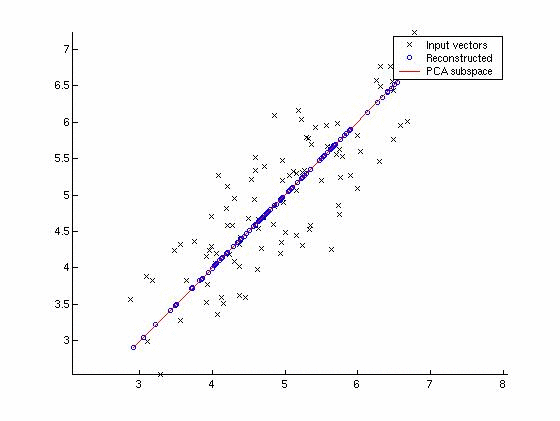
\includegraphics[width=\linewidth]{pca}
 \captionof{figure}{PCA}
\end{Figure}
Con la PCA vogliamo trovare una matrice di trasformazione \emph{W} tale che possiamo approssimare i campioni del dataset $x_i \in \rm I\!R^D$ con dei vettori $\hat{x_i}$ ottenuti da $\hat{x_i} = Wz_i$, ove $z_i \in \rm I\!R^L$ con $L<D$ e $W$ matrice ortogonale DxL. Vogliamo quindi minimizzare la distanza tra i campioni originali $x_i$ e le nostre approssimazioni $\hat{x_i}$, ossia matematicamente il \emph{reconstruction error}
\begin{equation}
\begin{split}
J(W,Z) &= \frac{1}{N}\sum_{i=1}^{N}|| x_i - Wz_i||^2\\
&= ||X^T - WZ^T||^2_F
\end{split}
\end{equation} 
dove $||A||_F$ identifica la \emph{Frobenius Norm}, ossia la radice della somma dei quadrati di tutti gli elementi della matrice.\\
Si osserva che la matrice $W$ che minimizza la norma di Frobenius è la matrice $V_L$ nella Singular Value Decomposition (SVD); infatti effettuando la SVD sulla Design Matrix $X$, si ottiene
\begin{equation}
\begin{split}
X &= USV^T
\implies
X_L = \color{gray}U_LS_L\color{violet}V_L^T\color{black} = \color{gray}Z\color{violet}W^T\color{black}\\
&ove\quad U_L^TU_L = I_L, \quad V_L^TV_L = I_D
\end{split}
\end{equation} 
con $S_L$ è la matrice diagonale contenente gli autovalori in ordine decrescente ottenuta da S ponendo a 0 le ultime $D-L$ componenti sulla diagonale. Infatti il \emph{reconstruction error} risulta pari a la somma dei $D - L$ autovalori esclusi:
\begin{equation}
\begin{split}
||X - X_L||_F &= ||U(S- \begin{bmatrix}
       S_L &     \\[0.3em]
          & 0  
     \end{bmatrix}) V^T ||_F\\ 
    &=||S- \begin{bmatrix}
       S_L &     \\[0.3em]
          & 0  
     \end{bmatrix} ||_F\\
     &=\sum_{i=L+1}^{D} \sigma_i
\end{split}
\end{equation}

\section{Visualizzazione dei dati}
In genere risulta estremamente utile effettuare una visualizzazione dei dati prima di procedere all'applicazione dei modelli, in modo da individuare pattern utili per guidare il processo di selezione del modello e l'analisi dei risultati ottenuti. I grafici in Figura 3 rappresentano le distribuzioni dei campioni considerando coppie di feature continue; ossia nella cella presente alla riga \emph{i-esima} e colonna \emph{j-esima} è presente un grafico in cui sull'asse x sono riportati i valori assunti dalla feature \emph{j-esima}, sull'asse y quelli assunti dalla feature \emph{i-esima} .

\begin{Figure}
 \centering
 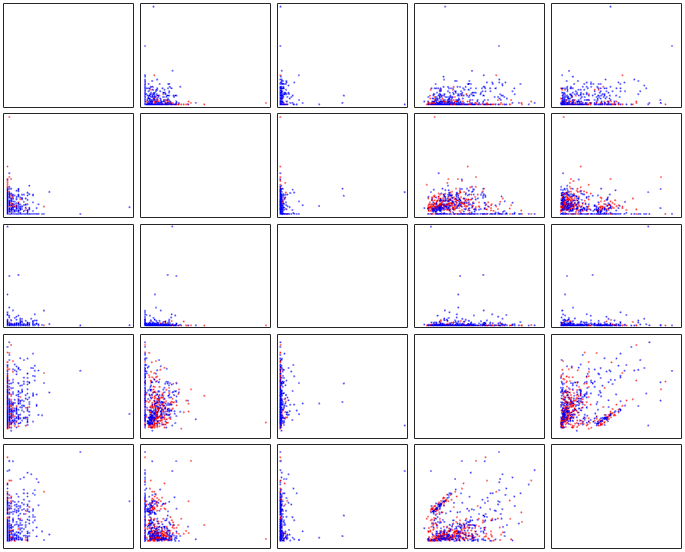
\includegraphics[width=\linewidth]{mcov}
 \captionof{figure}{}
\end{Figure}

Dai grafici non si evincono particolari legami tra le feature. E' pertanto necessario continuare ad investigare. %temporaneo...%
\section{Modelli utilizzati}
Si è deciso di affrontare il problema utilizzando diversi modelli, in modo da poter approfondire la struttura del problema proposto. Si è notato come modelli più semplici riescano a generalizzare maggiormente a fronte di nuovi dati di input, e ciò è dovuto a diversi fattori, tra cui la dimensione ridotta del dataset e il numero relativamente alto di feature.
Prima del training il dataset è stato inizialmente diviso in due parti: \emph{Training set} (80\%) e \emph{Test set} (20\%), utilizzati rispettivamente per il training e la selezione degli iperparametri attraverso la cross-validation e il test dei risultati ottenuti.\\
Nella Tabella 1 sono riportati gli error-rate medi e minimi ottenuti applicando i diversi modelli.\\
\begin{Table}
\small
   \begin{tabular}{|p{4.1cm}|p{0.8cm}|p{0.8cm}|}
\hline
 \multicolumn{1}{|c|}{\textbf{\scalebox{0.9}{Modello}}} & \multicolumn{1}{c}{\textbf{\scalebox{0.9}{Min}}} & \multicolumn{1}{|c|}{\textbf{\scalebox{0.9}{Med}}}\\ \hline
    	\scalebox{0.9}{Linear Discriminant Analysis}& 10.12 & 10 \\ \hline
	\scalebox{0.9}{Quadratic Discriminant Analysis} & 10 & 10\\ \hline
	\scalebox{0.9}{Diagonal Discriminant Analysis} & 0.04 & 0.224\\ \hline
\scalebox{0.9}{Logistic Regression (LB)} & 10 & 10 \\ \hline
	\scalebox{0.9}{Logistic Regression (QB)} & 10 & 10 \\ \hline
	\scalebox{0.9}{Logistic Regression (LBR)} & 10 & 10 \\ \hline
	\scalebox{0.9}{Logistic Regression (QBR)} & 10 & 10 \\ \hline
   \end{tabular}
  \captionof{table}{errori minimi e medi dei modelli utilizzati}
\end{Table}
\section{Gaussian Discriminant Analysis}
La Gaussian Discriminant Analysis, o GDA, è una tecnica di classificazione di tipo \emph{generativa}, e dunque calcola la distribuzione $p(x | y, \theta)$ (la class conditional density) di una serie di campioni, a partire dalla loro classe $y$ di appartenenza. Con la GDA, si assume che i campioni di ogni classe \emph{c} siano distribuiti come delle Gaussiane Multivariate, nel senso che
\begin{equation}
p(x|y=c) \sim \mathcal{N}(\mu_{c},\,\Sigma_{c})\quad \forall{c} \in \{1, ..., C\}
\end{equation}
dove $\mu_{c}$ rappresenta il vettore dei valori medi della distribuzione, e $\Sigma_{c}$ la matrice di covarianza delle feature.
%SCRIVI IL TEOREMA DI FREDA%
%DIFFERENZE TRA GENERATIVO E DISCRIMINATIVO%
Una volta trovati i due parametri $(\mu, \Sigma)$, per classificare un nuovo input $\hat{x}$ in una delle $C$ classi viene calcolato
\begin{equation}
\arg\max_{c}p(y = c|x = \hat{x}) \quad \forall{c} \in \{1, ..., C\}
\end{equation}
e cioè la massima probabilità che la classe di appartenenza di $\hat{x}$ sia \emph{c}, per tutte le $C$ classi.\\
Si osserva che indicando il prior con $\pi$, $\hat{y}(x)$ risulta:
\begin{equation}
\arg\max_{c}[\log{p(y=c|\pi_{c})} + \log{p(\hat{x}|y=c, \theta_{c})}]
\end{equation}
\begin{equation}
\arg\min_{c}[-\log{(\pi_{c})}+\frac{1}{2}\log{|\Sigma_{c}|} + \frac{1}{2}(\hat{x} - \mu_{c})^{T}\Sigma_{c}^{-1}(\hat{x} - \mu_{c})]
\end{equation}
L'ultimo parametro è la distanza di Mahalanobis al quadrato dal valore medio $\mu_{c}$ della classe $c$, ossia una distanza pesata con l'inverso degli autovalori di $\Sigma_{c}$ lungo i suoi autovettori:
\begin{equation}
\begin{split}
\Vert{x-\mu_{c}}\Vert_{\Sigma}^{2} &= (\hat{x} - \mu)^{T}\Sigma^{-1}(\hat{x} - \mu)\\
&=(\hat{x} - \mu)^{T}(\sum_{i=1}^{D} \frac{1}{\lambda_{i}}u_{i}u_{i}^{T})(\hat{x} - \mu)\\
&=\sum_{i=1}^{D} \frac{1}{\lambda_{i}}(\hat{x} - \mu)^{T}u_{i}u_{i}^{T}(\hat{x} - \mu)\\
&=\sum_{i=1}^{D} \frac{y_{i}^2}{\lambda_{i}}\\
ove\quad &y_{i} = \mu_{i}^T (x - \mu) 
\end{split}
\end{equation}
\begin{Figure}
 \centering
 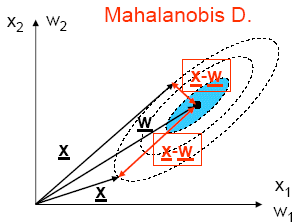
\includegraphics[width=\linewidth]{mahalanobis}
 \captionof{figure}{distanza di Mahalanobis}
\end{Figure}
\subsection{Quadratic Discriminant Analysis}
Ne consegue che il decision boundary tra due classi $(0,1)$ essendo definito come :
\begin{equation}
p(y = 0 | x) = p(y=1|x)
\end{equation}
corrisponde a :
\begin{equation}
( x-  \mu_0)^T \Sigma_0^{-1} (  x-  \mu_0) = ( x-  \mu_1)^T \Sigma_1^{-1} (  x-  \mu_1)\ + \ c
\end{equation}
Avendo un'equazione quadratica in entrambi i termini, nel caso generico il decision boundary si presenta come un paraboloide.
\begin{Figure}
 \centering
 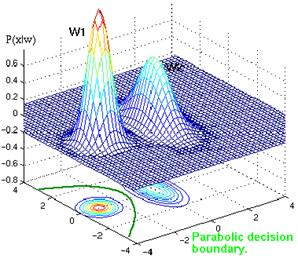
\includegraphics[width=\linewidth]{GDA}
 \captionof{figure}{Decision Boundary QDA}
\end{Figure}
\subsection{Linear Discriminant Analysis}
Assumendo che 
\begin{equation}
\Sigma_c = \Sigma \quad \forall \ c = \{1, ..., C\}
\end{equation}
\begin{equation}
\begin{split}
&p(y=c|{x}, \theta) \propto  \pi_c e^{-\frac{1}{2}({x} - \mu_{c})^{T}\Sigma^{-1}({x} - \mu_{c})}\\
&= e^{-\frac{1}{2}x^T\Sigma^{-1}x} e^{\mu_c^T\Sigma^{-1}x-\frac{1}{2}\mu_c^T\Sigma^{-1}\mu_c + \log\pi_c}\\
&\propto e^{-\frac{1}{2}\mu_c^T\Sigma^{-1}\mu_c + \log\pi_c}
\end{split}
\end{equation}
dove il primo termine è stato rimosso poiché non dipende dalla classe di appartenenza; poiché l'unico termine quadratico è stato rimosso, si possono evidenziare i termini $\gamma_c$ e $\beta_c$
\begin{equation}
\begin{split}
\gamma_c &= -\frac{1}{2}\mu_c^T\Sigma^{-1}\mu_c + \log\pi_c\\
\beta_c &= \Sigma^{-1}\mu_c
\end{split}
\end{equation}
ottenendo
\begin{equation}
p(y=c|{x}, \theta) \propto e^{\beta_c^Tx+\gamma_c}
\end{equation}
da cui si può evincere che il decision boundary è lineare
\begin{equation}
\begin{split}
p(y=c|{x}, &\theta) = p(y=c'|{x}, \theta) \\
&\iff \\
\beta_c^Tx+&\gamma_c = \beta_c'^Tx+\gamma_c'\\
& \iff\\
(\beta_c - \beta_{c'}&)^Tx = -(\gamma_c + \gamma_{c'})
\end{split}
\end{equation}
\begin{Figure}
 \centering
 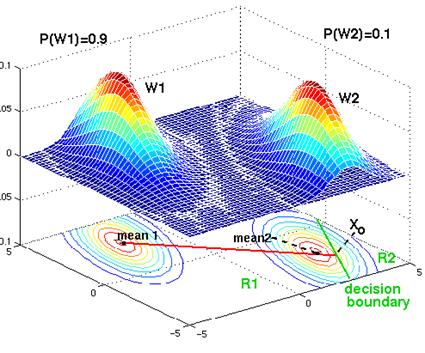
\includegraphics[width=\linewidth]{LDA}
 \captionof{figure}{Decision Boundary LDA}
\end{Figure}
\subsection{Diagonal Linear Discriminant Analysis}
Consideriamo il caso in cui $\Sigma_c = \Sigma = diag(\sigma_1^2, ..., \sigma_D^2) $ per ogni classe.
In tal caso gli autovettori di $\Sigma$ sono paralleli agli assi, e da quanto detto prima si deduce che $\hat{y}$ risulta pari a
\begin{equation}
\begin{split}
&\arg\min_{c}[-\log{(\pi_{c})}+ \frac{1}{2}(\hat{x} - \mu_{c})^{T}\Sigma^{-1}(\hat{x} - \mu_{c})]\\
&=\arg\min_{c}[-\log{(\pi_{c})}+\frac{1}{2}\sum_{i=1}^{D}\frac{(x_i - \mu_{ci})^2}{\sigma_i}]
\end{split}
\end{equation}
La Diagonal Linear Discriminant Analysis avendo meno parametri da stimare si comporta meglio in presenza di campioni con un alto numero di feature e dimensione del dataset ridotte, in quando tende a fare un minore overfitting.
\section{Logistic Regression}
La Logistic Regression è una tecnica di classificazione binaria di tipo \emph{discriminativo}, ossia si stima direttamente la $p(y|x)$ senza passare per class conditional density; in particolare si ottiene dalla \emph{Linear Regression} considerando le $y$ distribuite come una Bernulliana di parametro $\mu(x) = sigm(w^Tx)$.
\begin{equation}
y \sim Ber (y|\mu(x)), \quad \mu(x) = sigm(w^Tx)
\end{equation}
Differentemente dalla Linear Regression non è possibile trovare analiticamente con una formula chiusa il valore di w che minimizza p(D|w), e dunque è necessario utilizzare degli algoritmi di minimizzazione.
Calcolando la negative log-likelihood si ottiene infatti:
\begin{equation}
\begin{split}
NLL = &-log\ p(D|\theta) = \\
=\ &\sum_{i} [y_ilog( sigm(w^Tx)) \ + \\
&+\ (1- y_i)log(1 - sigm(w^Tx))  ]
\end{split}
\end{equation}


\subsection{Linear Boundary}
Dato che la
\begin{equation}
\begin{split}
&p(y|x,w) = Ber(y|sigm(w^Tx))\\
&=sigm(w^Tx)^{I(y=1)}(1-sigm(w^Tx))^{I(y=0)}
\end{split}
\end{equation}
allora ponendo $p(y=1|x,w) = p(y=0|x,w)$ per trovare il decision boundary si ottiene 
\begin{equation}
\begin{split}
sigm(w^Tx&)=(1-sigm(w^Tx)) \\
&\iff \\
sigm(w^Tx)&= 0.5 \implies w^Tx = 0
\end{split}
\end{equation}
che dunque risulta essere lineare.
\begin{Figure}
 \centering
 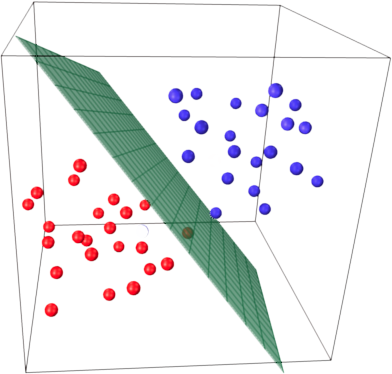
\includegraphics[width=\linewidth]{logL}
 \captionof{figure}{Linear Boundary Logistic Regression}
\end{Figure}


\subsection{Quadratic Boundary}
Per ottenere un boundary non lineare si può sostituire ai campioni $x$ un vettore $\phi(x)$ che contiene funzioni della x; in particolare con un ragionamento analogo a quello utilizzato nel caso lineare si osserva che il decision boundary sarà dato da
\begin{equation}
w^T\phi(x) = 0
\end{equation}
Dunque, utilizzando una \textbf{multivariate polynomial expansion} di grado 2, è possibile ottenere un boundary quadratico.
\begin{equation}
w^T\phi(x) = w_0 + \sum_{i=1}^{D} w_i x_i + \sum_{i,j : i<=j}^{D} w_{ij}x_{i}x_j 
\end{equation}
\begin{Figure}
 \centering
 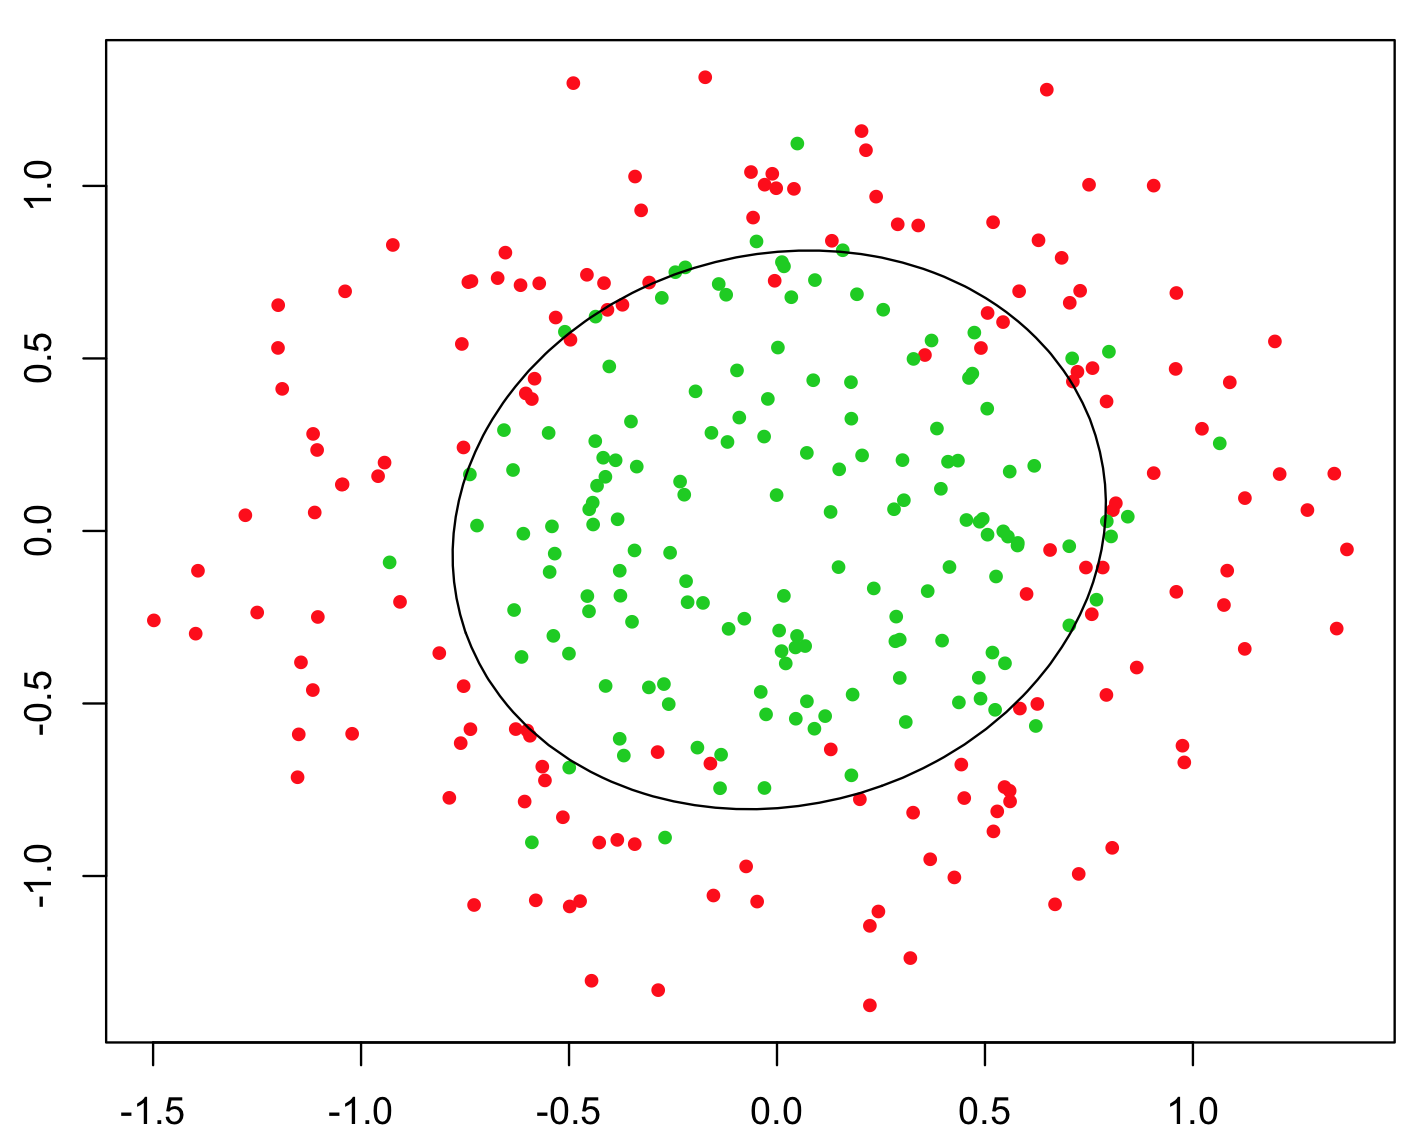
\includegraphics[width=\linewidth]{quadratic}
 \captionof{figure}{Quadratic Boundary Logistic Regression}
\end{Figure}


\subsection{Regolarizzazione}
In presenza di un dataset ristretto e di molti parametri in un modello, ad esempio utilizzando un polinomio di grado alto, è possibile che i parametri trovati dal modello non generalizzino bene a fronte di nuovi dati di input, ossia è facile che il modello faccia overfitting sul training set; in questi casi i valori assunti da $w$ sono specifici per i dati in ingresso e tendono a fittare anche il rumore, facendo assumere a $w$ dei coefficienti elevati per poter seguire tutte le variazioni di quest'ultimo.\\
Un modo per limitare la flessibilità del modello rispetto al rumore, e in tal modo ridurre l'overfitting consiste nell'aggiungere dei pesi ai coefficienti $w$, in modo tale che durante la minimizzazione dell'errore, questi tendano a non assumere valori troppo elevati.\\
Tali pesi possono essere espressi come un prior su $w$, distribuito come una normale di centro 0 e varianza $\lambda$, in modo da poter influenzare la distribuzione di probabilità $p(w|D)$
\begin{equation}
p(w) = \mathcal{N}(0, \lambda I) \quad p(w|D) \propto p(D|w)p(w)
\end{equation}
da cui la funzione da minimizzare diventa
\begin{equation}
f(w) = NLL(w) + \lambda w^Tw
\end{equation}
\section{Bias vs Variance}
Quando si parla di \emph{prediction error}, questo può essere decomposto in tre componenti: errore dovuto al \emph{bias}, errore dovuto alla \emph{varianza} ed errore irriducibile dovuto al rumore. E' importante individuare quali sono le componenti d'errore nel nostro modello, per poter comprendere come questo si stia comportando e se stia effettuando under o over-fitting.
Il \emph{Bias} e la \emph{Variance} sono definiti a livello matematico come:
\begin{equation}
\begin{split}
Bias &= E[\hat{f}(x)]-f(x)\\
Variance &= E\left[\left(\hat{f}(x)-E[\hat{f}(x)]\right)^2\right]
\end{split}
\end{equation}
Intuitivamente il Bias rappresenta l'errore sulla media delle nostre predizioni per ogni campione del dataset, supponendo di effettuare il training del modello con diversi dataset, mentre la Variance rappresenta quanto variano le nostre predizioni tra di loro per un dato campione.\\
In genere vorremmo avere Bias e Variance nulli, ossia vorremmo predire sempre il valore corretto, ma ci si rende conto che esiste un trade-off tra le due fonti di errore, infatti si può intuire una correlazione tra Bias/Variance e Underfitting/Overfitting: più il nostro modello farà overfitting sul training set, più varieranno le predizioni al variare dei dati in input e dunque si avrà un'alta Variance; d'altra parte facendo underfitting le nostre predizioni saranno meno influenzate dai dati in input e quindi avranno una bassa variance ed un alto Bias, poiché lo stesso errore si ripeterà sistematicamente.\\
Indicando nel cerchio rosso il valore corretto della y e con i pallini blu le nostre predizioni, possiamo graficare diverse combinazioni di Bias e Variance nel seguente modo
\begin{Figure}
 \centering
 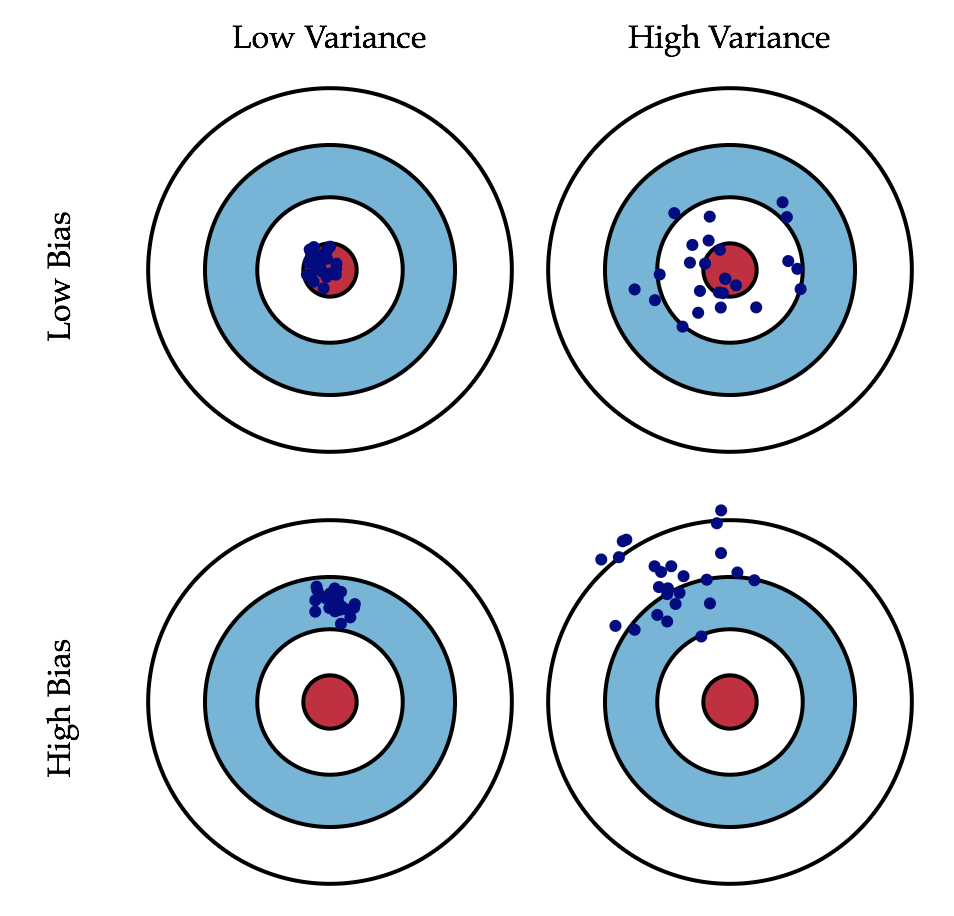
\includegraphics[width=\linewidth]{BiasVariance}
 \captionof{figure}{Interpretazione grafica Bias/Variance}
\end{Figure}
\end{multicols}

\begin{thebibliography}{10}
\bibitem{Dataset}
	John Ross Quinlan \\
	\emph{Credit Approval Data Set} \\
	\url{http://archive.ics.uci.edu/ml/datasets/Credit+Approval}
\bibitem{OneHotEncoding}
	Håkon Hapnes Strand \\
	\emph{One Hot Encoding} \\
	\url{https://www.quora.com/What-is-one-hot-encoding-and-when-is-it-used-in-data-science}
	
\end{thebibliography}

\begin{equation}
\end{equation}

\end{document}